\section{Lektion 03-04-2018}

\begin{enumerate}
	\item Oscillatorer
	\item Colpitts
	\item Seiler
	\item Pierce
	\item Krystal Oscillatorer
\end{enumerate}

\begin{mdframed}[style=exampledefault]
	\begin{itemize}
		\item \textbf{Pensum:} CB, Ch 8 p. 190-191. JV, Ch 6 p. 1-8, 15-19, 35-46
		\item \textbf{Opgaver:} 
		\begin{itemize}
			\item Ex2007 opg. 1
			\item Lektion 7-1
			\item Ex2011/12 opg. 1
			\item Ex2013 opg. 1
			item Ex2013 opg. 1
			\item Opg. Øv.1
		\end{itemize}
	\end{itemize}
\end{mdframed}

\subsection{Oscillatorer}
\begin{itemize}
	\item Local Oscillators are often a phase-locked voltage-controlled oscillator (VCO).
	\item LO is capable of covering the frequency range of interest for
	translating incoming RF signals to a desired IF range.
\end{itemize}

\subsection{LC Oscillatorer}
\begin{itemize}
	\item Circuits intended for sinusoidal outputs up to a few \si{\giga\hertz} in frequency may be build using inductors and capacitors as tuning elements.
	\item Q-factor determines properties of frequency stability and noise in the oscillator.
\end{itemize}

\begin{equation}
Q_l = \dfrac{\omega_0}{2}\left|\dfrac{d\angle A_{ol}}{d\omega}\right|_{\omega_0}
\end{equation}

\begin{itemize}
	\item Loading of the transistor might have to be checked whether or not a device is adequate in a given application.
\end{itemize}

\begin{equation}
Z_{lt}=\dfrac{V_{a1}}{-G_mV_{b1}}=\dfrac{-1}{G_m}\left(\dfrac{Y_b}{Y_c}+1\right)
\end{equation}

\begin{figure} [H]
	\centering
	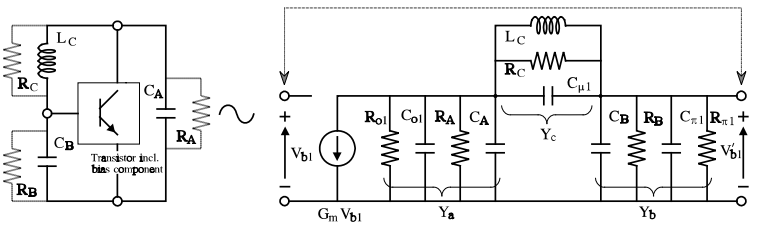
\includegraphics[width=\linewidth]{graphics/48.png}
	\caption{LC oscillator/equivalent circuit includes the large signal transistor model. Resistors $R_A$, $R_B$, and $R_C$ represent losses and/or loads.}
	\label{fig:48}
\end{figure}

\begin{itemize}
	\item Colpitt's, Pierce, and Seiler oscillators are deduced by grounding base, emitter, or collector - gate, source, or drain - respectively.
	\item The transistor symbol represents a transistor under large signal operation.
	\item Includes the type of bias network that is required to reduce transconductance and in turn stabilize the oscillation amplitude.
\end{itemize}

\subsubsection{Colpitts}
\begin{figure} [H]
	\centering
	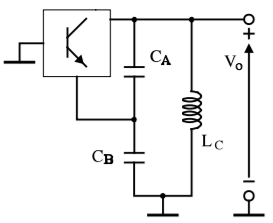
\includegraphics[width=0.45\linewidth]{graphics/42.png}
	\caption{Colpitts oscillator.}
	\label{fig:42}
\end{figure}

\subsubsection{Seiler}
\begin{figure} [H]
	\centering
	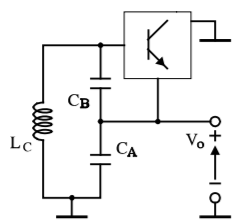
\includegraphics[width=0.4\linewidth]{graphics/43.png}
	\caption{Seiler oscillator.}
	\label{fig:43}
\end{figure}

\subsubsection{Pierce}
\begin{figure} [H]
	\centering
	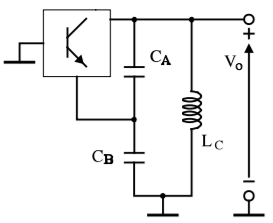
\includegraphics[width=0.45\linewidth]{graphics/42.png}
	\caption{Pierce oscillator.}
	\label{fig:44}
\end{figure}

\subsection{Krystal Oscillatorer}
\begin{itemize}
	\item Oscillator where a crystal have replaced inductor of a LC circuit.
	\item Optional series capacitor may be inserted to tune	frequency and/or transform impedance levels.
\end{itemize}
\subsubsection{Colpit}
\begin{figure} [H]
	\centering
	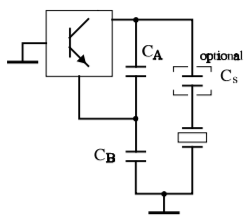
\includegraphics[width=0.45\linewidth]{graphics/45.png}
	\caption{Colpitts oscillator.}
	\label{fig:45}
\end{figure}

\subsubsection{Seiler}
\begin{figure} [H]
	\centering
	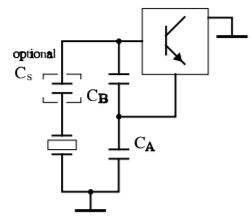
\includegraphics[width=0.45\linewidth]{graphics/46.png}
	\caption{Seiler oscillator.}
	\label{fig:46}
\end{figure}

\subsubsection{Pierce}
\begin{figure} [H]
	\centering
	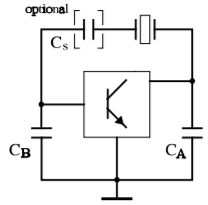
\includegraphics[width=0.4\linewidth]{graphics/47.png}
	\caption{Pierce oscillator.}
	\label{fig:47}
\end{figure}